\begin{figure}[htb!]
    \centering
    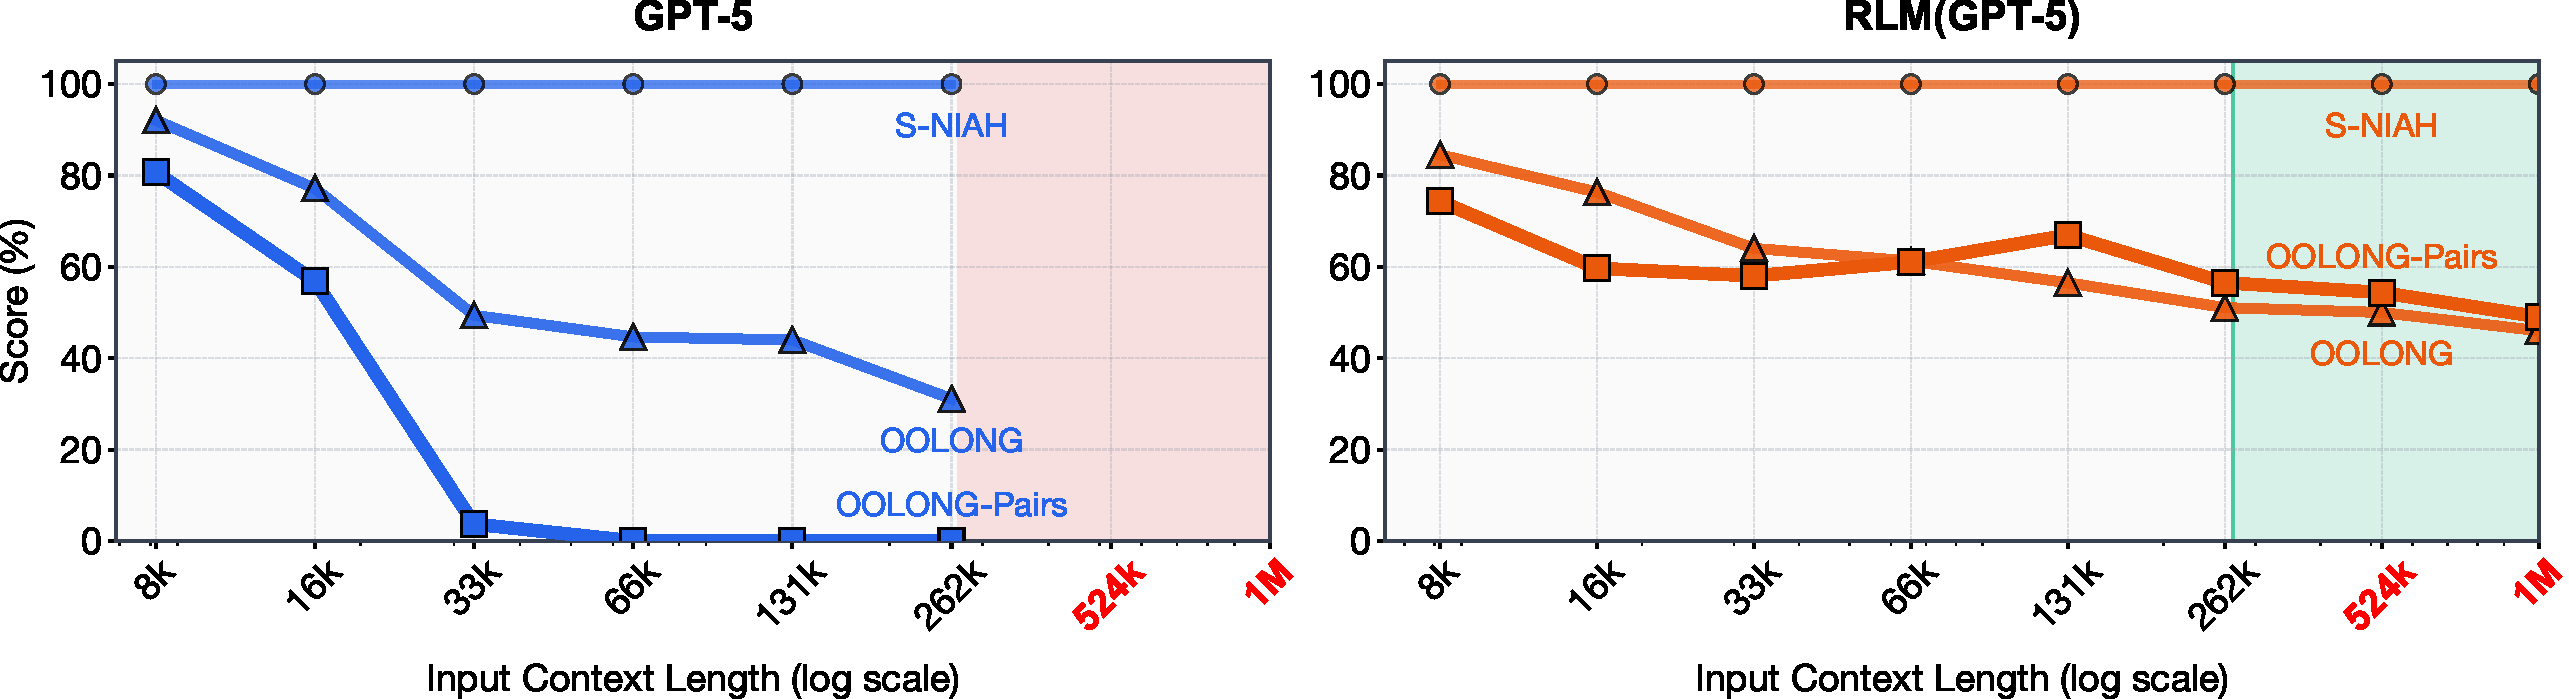
\includegraphics[width=\textwidth]{figures/scaling_plot.pdf}
    \caption{A comparison of GPT-5 and a corresponding \RLM{} on three long-context tasks of increasing complexity: \textbf{S-NIAH}, \textbf{OOLONG}, and \textbf{OOLONG-Pairs}. For each task, we scale the input length from $2^{13}$ to $2^{18}$. GPT-5 performance degrades significantly as a function of both input length and task complexity, while the \RLM{} maintains strong performance.
     Inputs beyond the red region do not fit in GPT-5's context window of 272K tokens, but the \RLM{} handles them effectively. Additional experiments across other models, methods, and benchmarks are in \S\ref{sec4:long-input}.}
    \label{fig:rlm-scaling}
\end{figure}


Despite rapid progress in reasoning and tool use, modern language models still have limited context lengths and, even within these limits, appear to inevitably exhibit \textit{context rot}~\citep{hong2025contextrot}, the phenomenon illustrated in the left-hand side of Figure~\ref{fig:rlm-scaling} where the quality of even frontier models like GPT-5 degrades quickly as context gets longer. Though we expect context lengths to steadily rise through improvements to training, architecture, and infrastructure, we are interested in \textit{whether it possible to dramatically scale the context size of general-purpose LLMs by orders of magnitude}. This is increasingly urgent as LLMs begin to be widely adopted for long-horizon tasks, in which they must routinely process tens if not hundreds of millions of tokens.

We study this question through the lens of scaling inference-time compute. We draw broad inspiration from \textit{out-of-core} algorithms, in which data-processing systems with a small but fast main memory can process far larger datasets by cleverly managing how data is fetched into memory. Inference-time methods for dealing with what are in essence long-context problems are very common, though typically task-specific. One general and increasingly popular inference-time approach in this space is context condensation or compaction \citep{khattab2021baleen,smith2025openhands_context_condensensation,openai_codex_cli,wu2025resumunlockinglonghorizonsearch}, in which the context is repeatedly summarized once it exceeds a length threshold. Unfortunately, compaction is rarely expressive enough for tasks that require dense access to many parts of the prompt, as it presumes in effect that \textit{some} details that appear early in the prompt can safely be forgotten to make room for new content.





\begin{figure}[t]
    \centering
    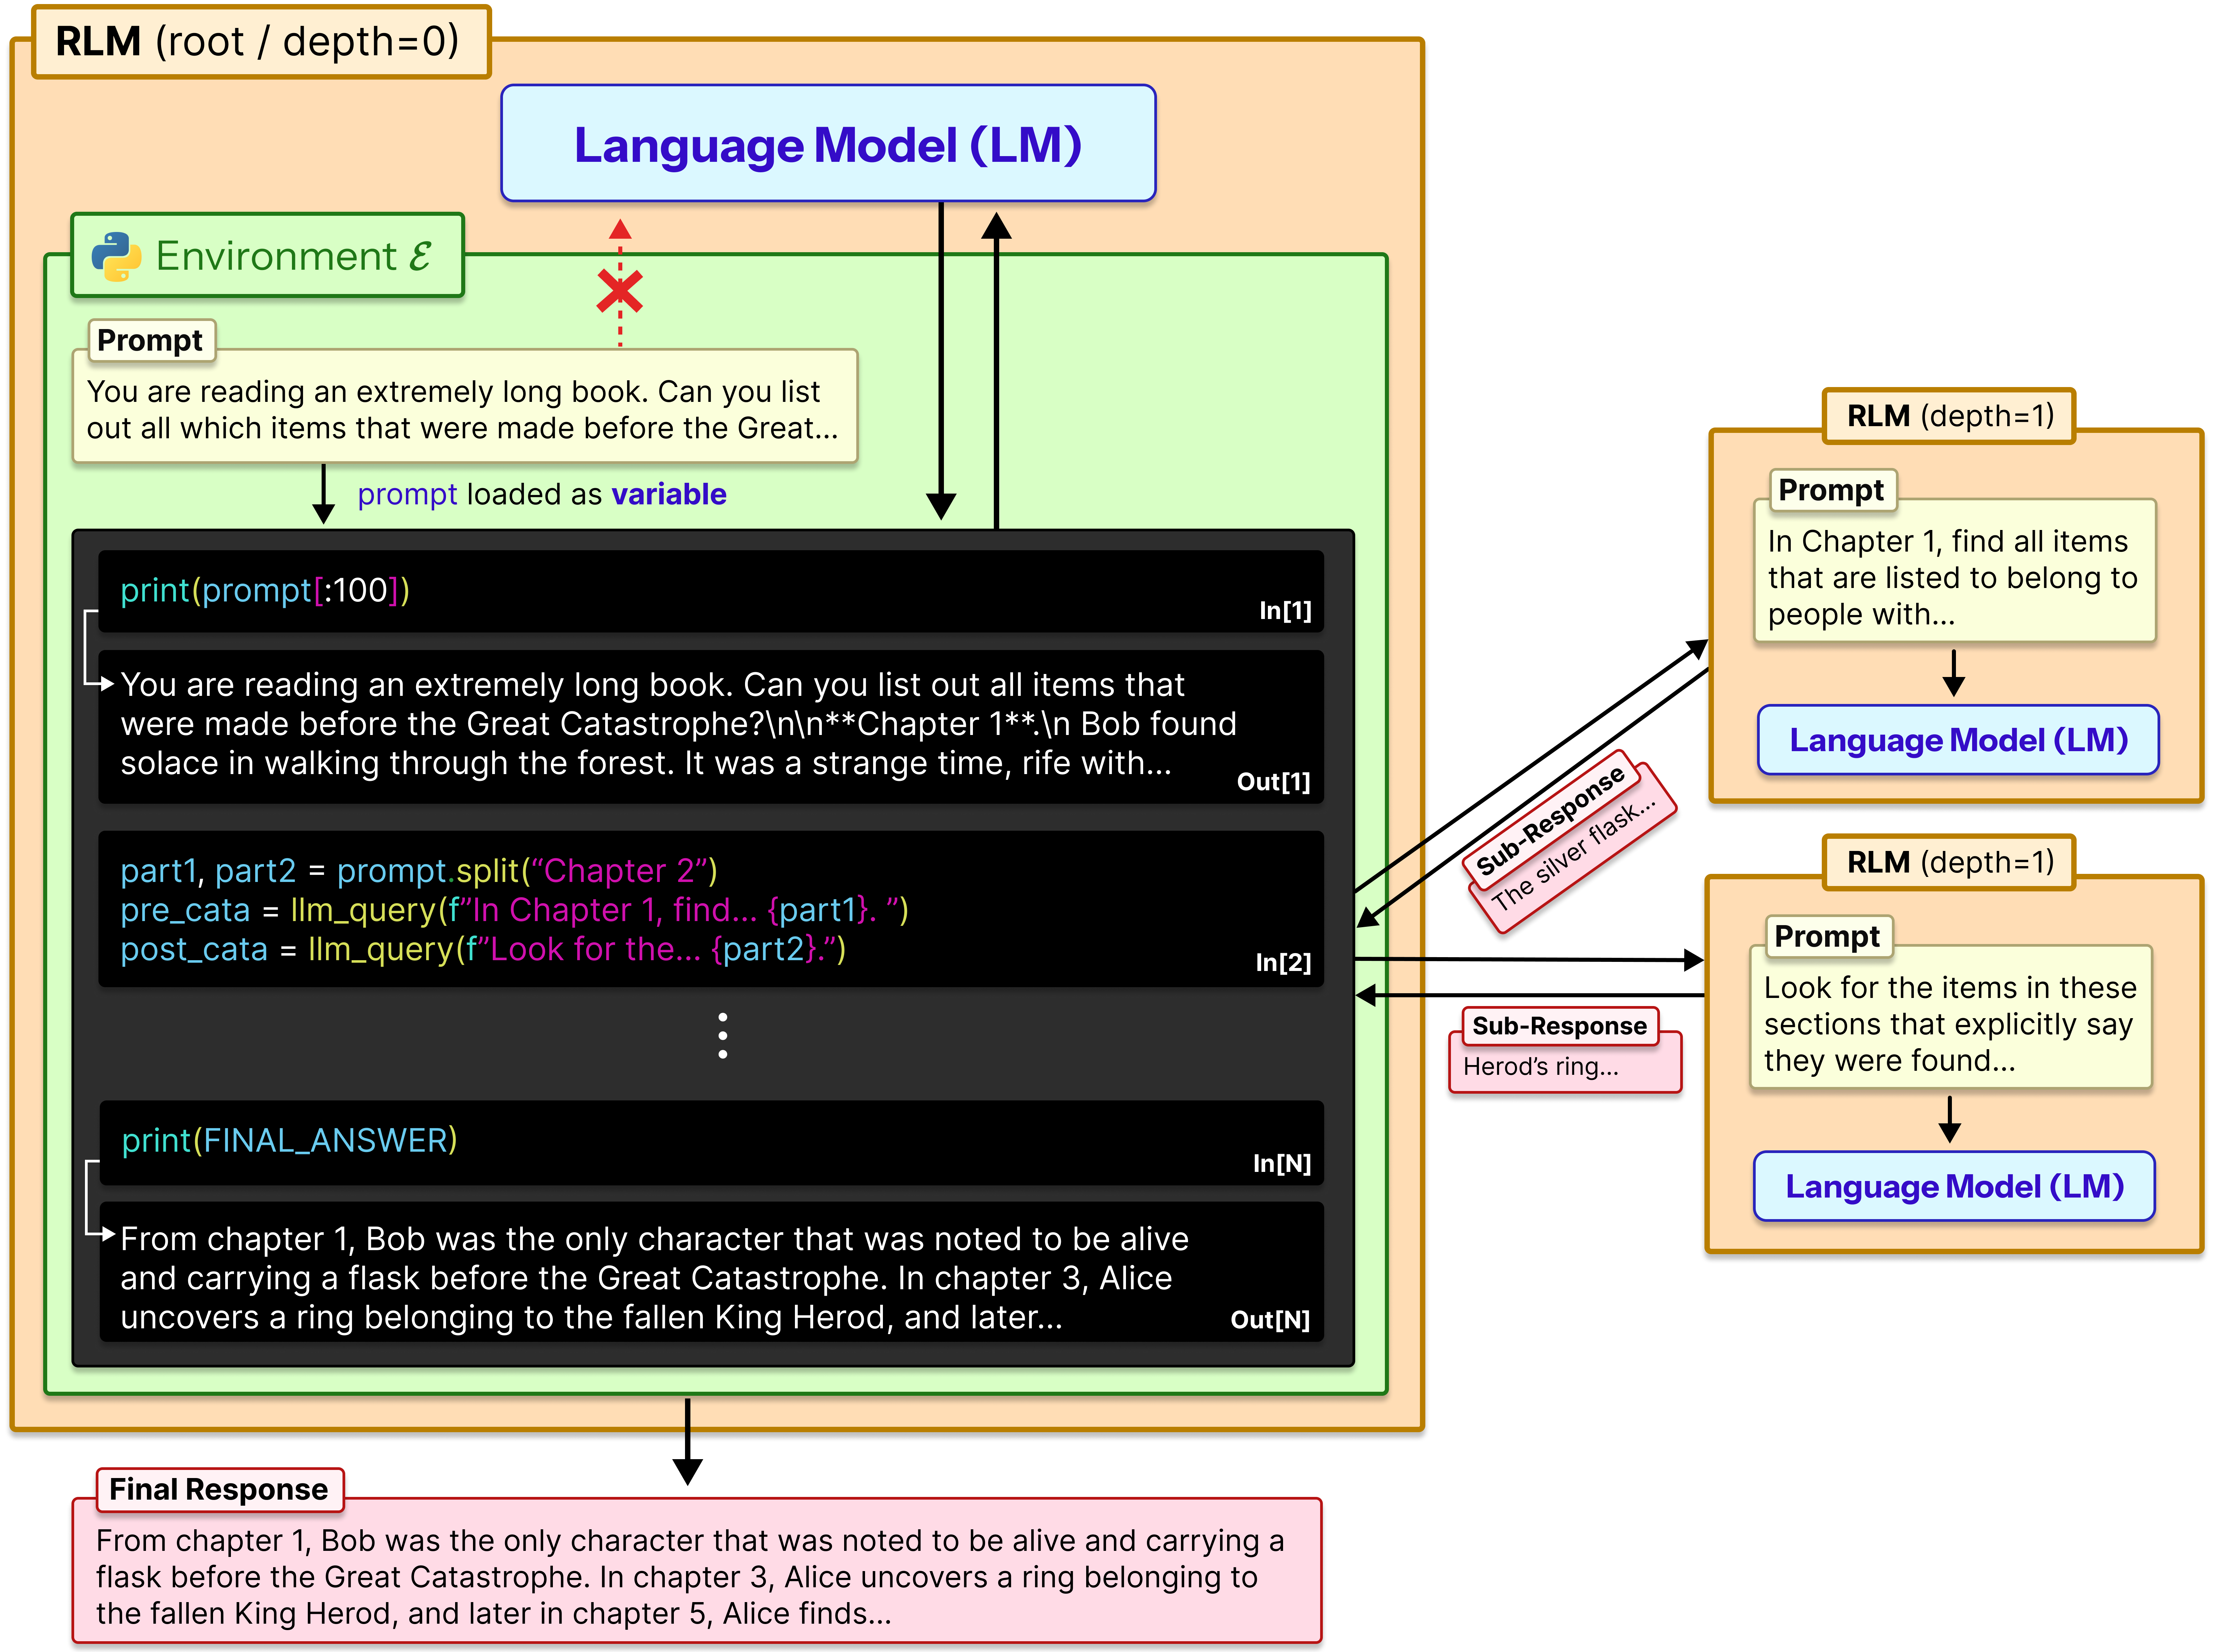
\includegraphics[width=0.93\textwidth]{figures/Fig2.png}
    \caption{A Recursive Language Model (\RLM{}) treats prompts as part of the environment. It loads the input prompt as a variable inside a Python REPL environment $\mathcal{E}$ and writes code to peek into, decompose, and invoke itself recursively over programmatic snippets of the variable.}
    \label{fig:rlm-repl}
    \vspace{-1em}
\end{figure}

We introduce \textbf{Recursive Language Models} (\textbf{\RLM{}}s), a general-purpose inference paradigm for dramatically scaling the effective input and output lengths of modern LLMs. The key insight is that long prompts should not be fed into the neural network (e.g., Transformer) directly but should instead be treated as \textit{part of the environment that the LLM can symbolically interact with}.

As Figure~\ref{fig:rlm-repl} illustrates, an RLM exposes the same external interface as an LLM: it accepts a string prompt of arbitrary structure and produces a string response. Given a prompt $P$, the RLM initializes a Read-Eval-Print Loop (REPL) programming environment in which $P$ is set as the value of a variable. It then offers the LLM general context about the REPL environment (e.g., the length of the string $P$), and permits it to write code that peeks into and decomposes $P$, and to iteratively observe any side effects from execution. Crucially, RLMs encourage the LLM, in the code it produces, to programmatically construct sub-tasks on which they can invoke themselves recursively.

By treating the prompt as an object in the external environment, this simple design of RLMs tackles a foundational limitation in the many prior approaches~\citep{anthropic_claude_code_subagents,sentient2025roma,schroeder2025threadthinkingdeeperrecursive, sun2025scalinglonghorizonllmagent}, which focus on recursive decomposition of the \textit{tasks} but cannot allow their input to scale beyond the context window of the underlying LLM.

We evaluate \RLM{}s using a frontier closed model (GPT-5;~\citealt{openai2025gpt5systemcard}) and a frontier open model (Qwen3-Coder-480B-A35B;~\citealt{Qwen3-Coder-480B-A35B}) across four diverse tasks with varying levels of complexity for deep research~\citep{chen2025browsecompplusfairtransparentevaluation}, information aggregation~\citep{bertsch2025oolongevaluatinglongcontext}, code repository understanding~\citep{bai2025longbenchv2deeperunderstanding}, and a synthetic pairwise reasoning task where even frontier models fail catastrophically. We compare RLMs against direct LLM calls as well as context compaction, retrieval tool-use agents, and code-generation agents.
We find that RLMs demonstrate extremely strong performance even at the 10M+ token scale, and dramatically outperform all other approaches at long-context processing, in most cases by double-digit percentage gains while maintaining a comparable or lower cost. In particular, as demonstrated in Figure~\ref{fig:rlm-scaling} exhibit far less severe degradation for longer contexts and more sophisticated tasks.




